\documentclass[11 pt]{exam}
\usepackage[lmargin=1in,rmargin=1.75in,bmargin=1in,tmargin=1in]{geometry}

% For hyperlinking everything
\usepackage{hyperref}
\hypersetup{
	colorlinks=true, %set true if you want colored links
	linktoc=all,     %set to all if you want both sections and subsections linked
	linkcolor=blue,  %choose some color if you want links to stand out
}


\usepackage[latin1]{inputenc}
\usepackage{amsmath}
\usepackage{mathrsfs}  
\usepackage{amsfonts}
\usepackage{amssymb}
\usepackage{graphicx}
\usepackage{subfig}
\usepackage{caption}
\usepackage{algorithm}
%\usepackage{algcompatible}
%\usepackage{algorithmicx}
\usepackage{algpseudocode}

\usepackage{titlesec}
\titleformat{\section}{\fontfamily{lmss}\fontsize{14}{15}\bfseries}{\thesection}{1em}{}
\titleformat{\subsection}{\fontfamily{lmss}\fontsize{12}{15}\bfseries}{\thesubsection}{1em}{}




\usepackage{amsthm}

\newtheoremstyle{noit}
{10pt}% <Space above>
{10pt}% <Space below>
{}% <Body font>
{}% <Indent amount>
{\bfseries}% <Theorem head font>
{.}% <Punctuation after theorem head>
{.5em}% <Space after theorem headi>
{}% <Theorem head spec (can be left empty, meaning `normal')>

\newtheoremstyle{example}
{10pt}% <Space above>
{10pt}% <Space below>
{}% <Body font>
{20pt}% <Indent amount>
{\bfseries}% <Theorem head font>
{.}% <Punctuation after theorem head>
{.5em}% <Space after theorem headi>
{}% <Theorem head spec (can be left empty, meaning `normal')>


\newtheoremstyle{indented}{20pt}{20pt}{\addtolength{\leftskip}{2.5em}}{}{\bfseries}{.}{.5em}{}


\newtheorem{theorem}{Theorem}
\numberwithin{theorem}{section}
\newtheorem{lemma}[theorem]{Lemma}
\newtheorem{corollary}[theorem]{Corollary}
\newtheorem{observation}{Observation}
%\numberwithin{observation}{section}
%\numberwithin{definition}{section}
\newtheorem{conjecture}{Conjecture}
\newtheorem{Qu}{Question}
\newcommand{\QU}{\begin{Qu}\normalfont}

\theoremstyle{noit}
\newtheorem{fact}{Fact}
\newtheorem{definition}{Definition}

\theoremstyle{indented}
\newtheorem{example}{Example}

\theoremstyle{indented}
\newtheorem{problem}{Problem}


%\newenvironment{proof}{\noindent{\bf Proof:} \hspace*{1em}}{
%    \hspace*{\fill} $\Box$ }
%\newenvironment{proof_of}[1]{\noindent {\bf Proof of #1:}
%    \hspace*{1em} }{\hspace*{\fill} $\Box$ }
%\newenvironment{proof_claim}{\begin{quotation} \noindent}{
%    \hspace*{\fill} $\diamond$ \end{quotation}}
\newcommand{\vs}[1]{\vspace{#1}}

\newcommand{\lecture}[2]{
 \noindent
\begin{center}
	\framebox{
		\vbox{
			\hbox to 5.78in { {\bf CSCE 411: Design and Analysis of Algorithms (Honors)} \hfill  }
			\vspace{2mm}
			\hbox to 5.78in { {\Large \hfill Lecture #1\hfill} }
			\vspace{2mm}
			\hbox to 5.78in { {\it Date: #2 \hfill Samson Zhou} }
		}
	}
\end{center}
\vspace*{4mm}
}

\newcommand{\week}[2]{
 \noindent
\begin{center}
	\framebox{
		\vbox{
			\hbox to 5.78in { {\bf CSCE 411: Design and Analysis of Algorithms (Honors)} \hfill  }
			\vspace{2mm}
			\hbox to 5.78in { {\Large \hfill Week #1\hfill} }
			\vspace{2mm}
			\hbox to 5.78in { {\it Date: #2 \hfill Nate Veldt, updated by Samson Zhou} }
		}
	}
\end{center}
\vspace*{4mm}
}

\newcommand{\sweek}[2]{
 \noindent
\begin{center}
	\framebox{
		\vbox{
			\hbox to 5.78in { {\bf CSCE 411: Design and Analysis of Algorithms (Honors)} \hfill  }
			\vspace{2mm}
			\hbox to 5.78in { {\Large \hfill Week #1\hfill} }
			\vspace{2mm}
			\hbox to 5.78in { {\it Date: #2 \hfill Samson Zhou} }
		}
	}
\end{center}
\vspace*{4mm}
}

\newcommand{\hw}[2]{
	\noindent
	\begin{center}
		\framebox{
			\vbox{
				\hbox to 5.78in { {\bf CSCE 411: Design and Analysis of Algorithms} \hfill  }
				\vspace{2mm}
				\hbox to 5.78in { {\Large \hfill Homework #1\hfill} }
				\vspace{2mm}
				\hbox to 5.78in { {\it Due date: #2 \hfil} }
			}
		}
	\end{center}
	\vspace*{4mm}
}



\newcommand{\under}[1]{\underline{\hspace{#1}}}
\setlength{\parindent}{0em}

%\usepackage[tagged]{accessibility}

% Graph terms
\newcommand{\vol}{\textbf{vol}}
\newcommand{\cut}{\textbf{cut}}


% Matrices
\newcommand{\mA}{\textbf{A}}
\newcommand{\mB}{\textbf{B}}

% vectors
\newcommand{\ve}{\textbf{e}}
\newcommand{\vx}{\textbf{x}}


% Other
\newcommand{\calN}{\mathcal{N}}

\usepackage{mathtools}
\DeclarePairedDelimiter\ceil{\lceil}{\rceil}
\DeclarePairedDelimiter\floor{\lfloor}{\rfloor}


\newcommand*{\aitem}{ \item[{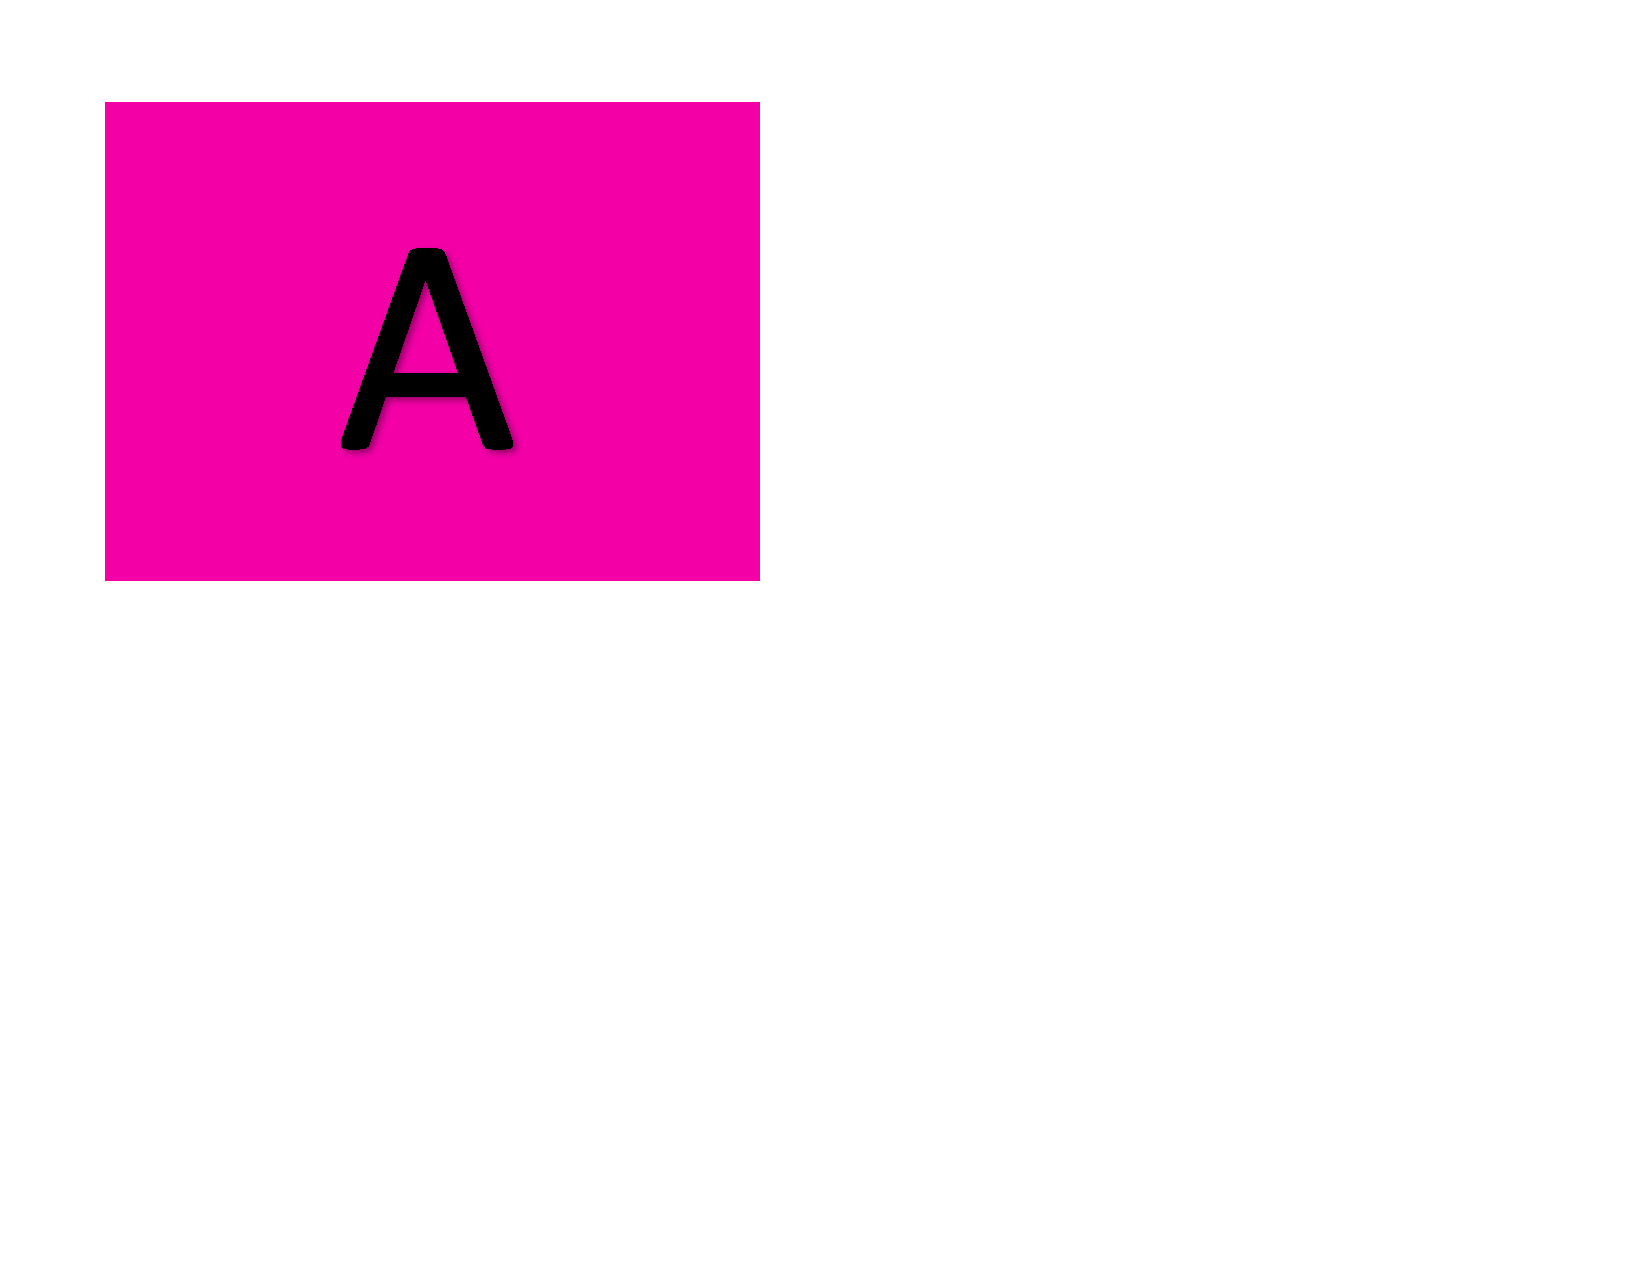
\includegraphics[width=0.8cm,height=0.5cm]{figures/A}} ]  }
\newcommand*{\bitem}{ \item[{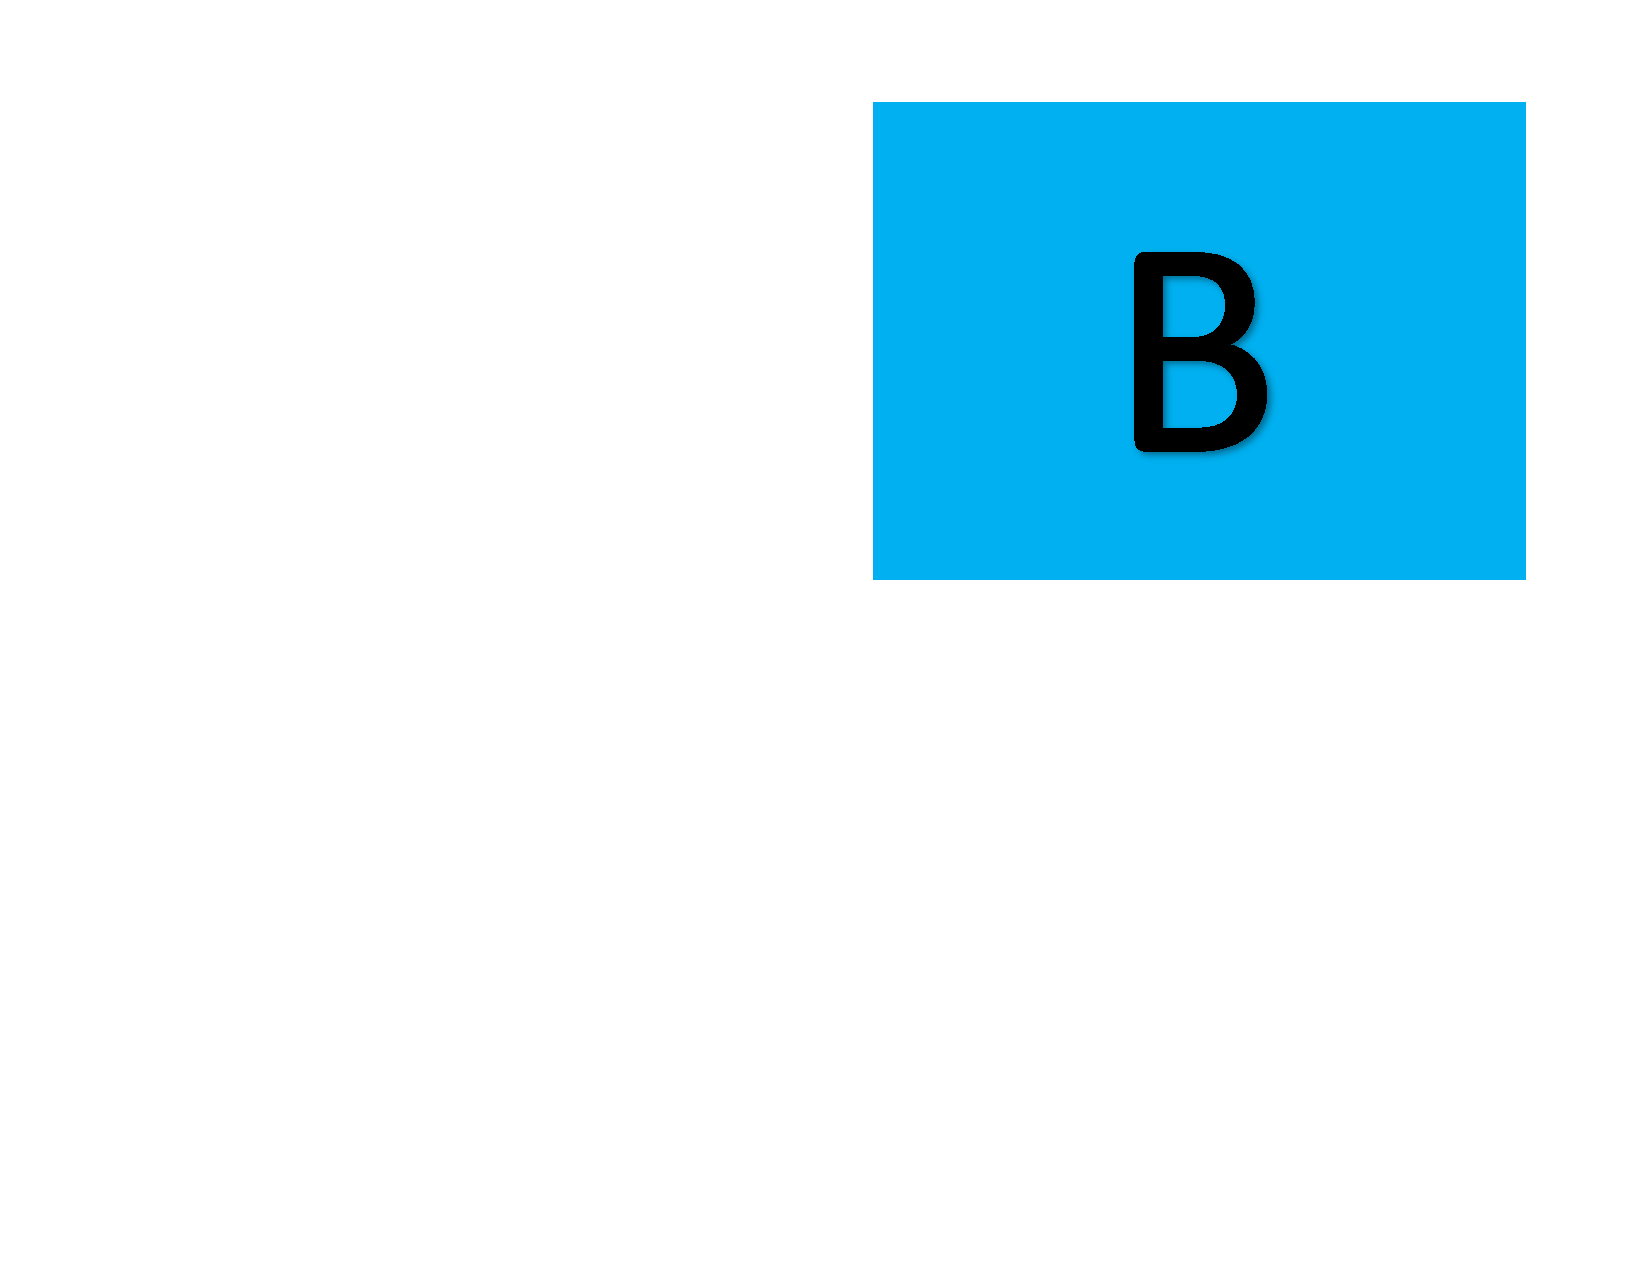
\includegraphics[width=0.8cm,height=0.5cm]{figures/B}} ]  }
\newcommand*{\citem}{ \item[{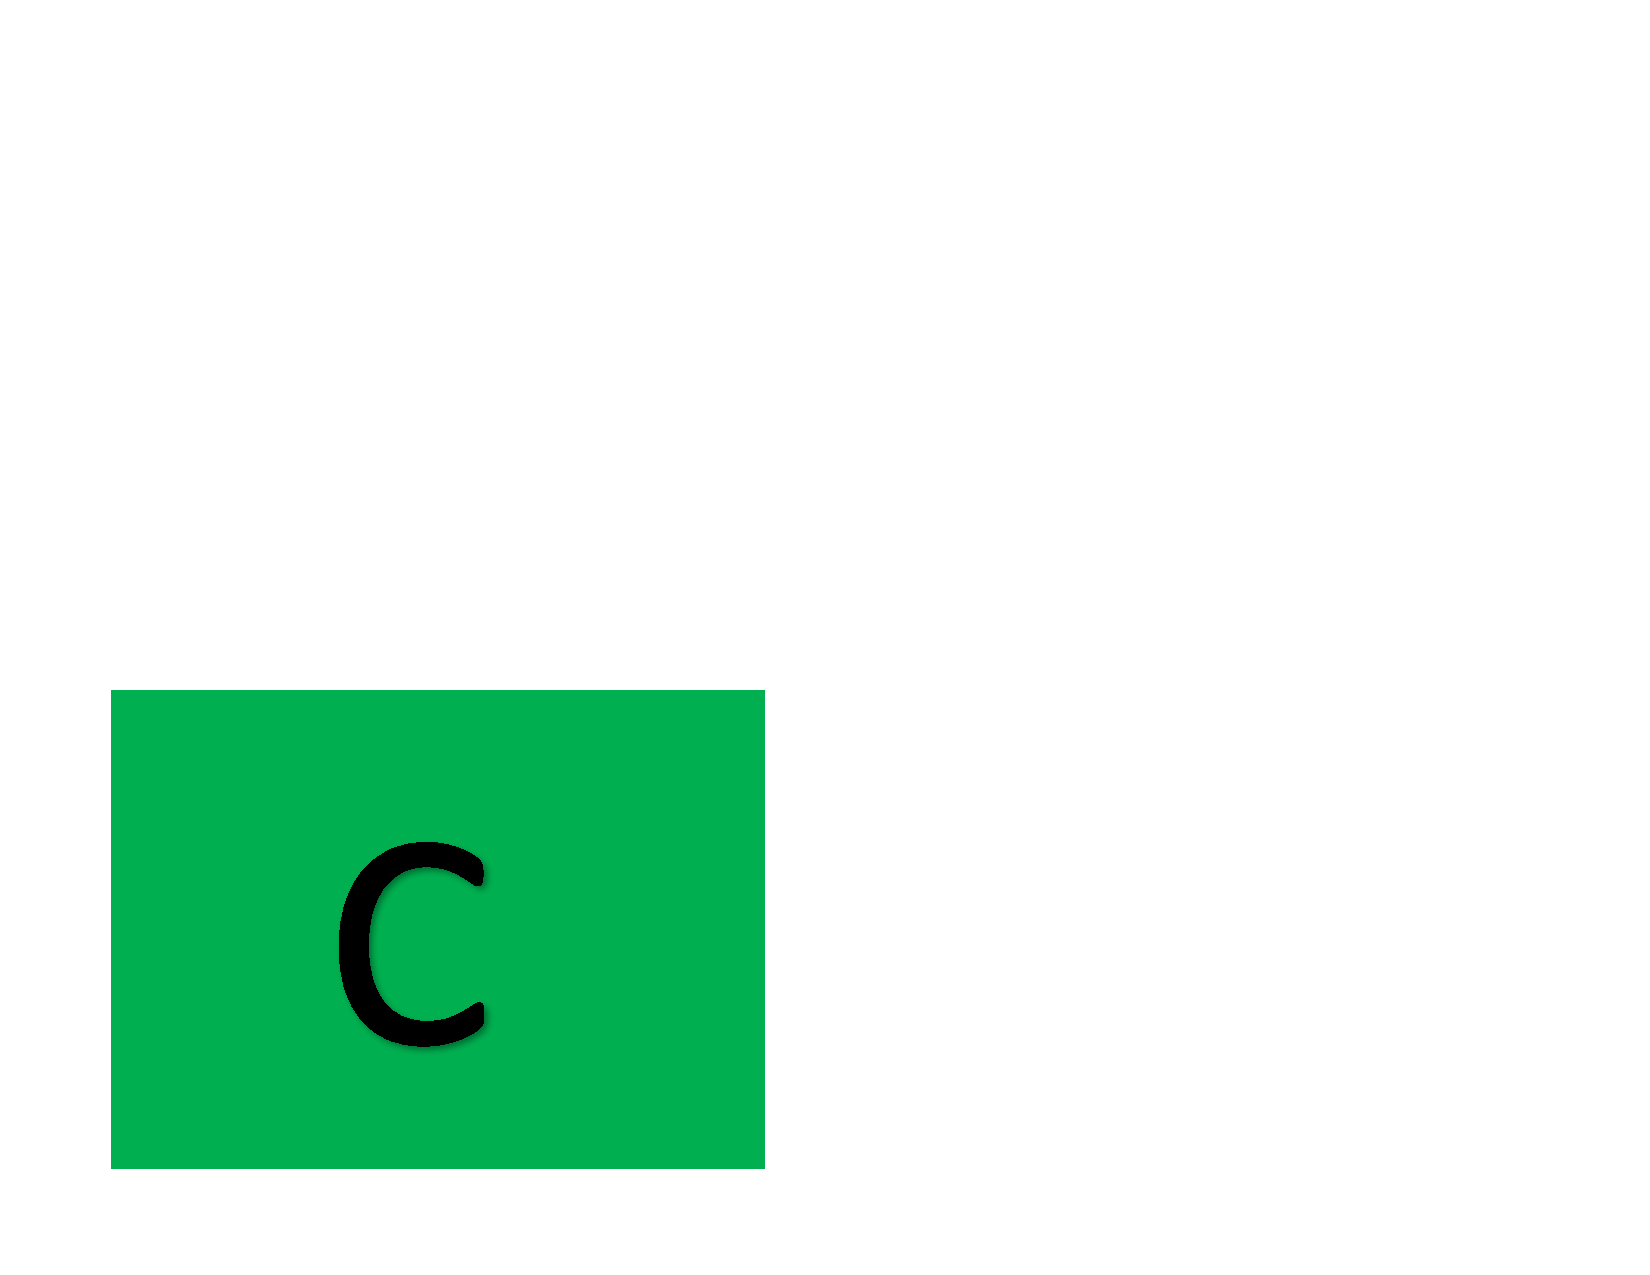
\includegraphics[width=0.8cm,height=0.5cm]{figures/C}} ]  }
\newcommand*{\ditem}{ \item[{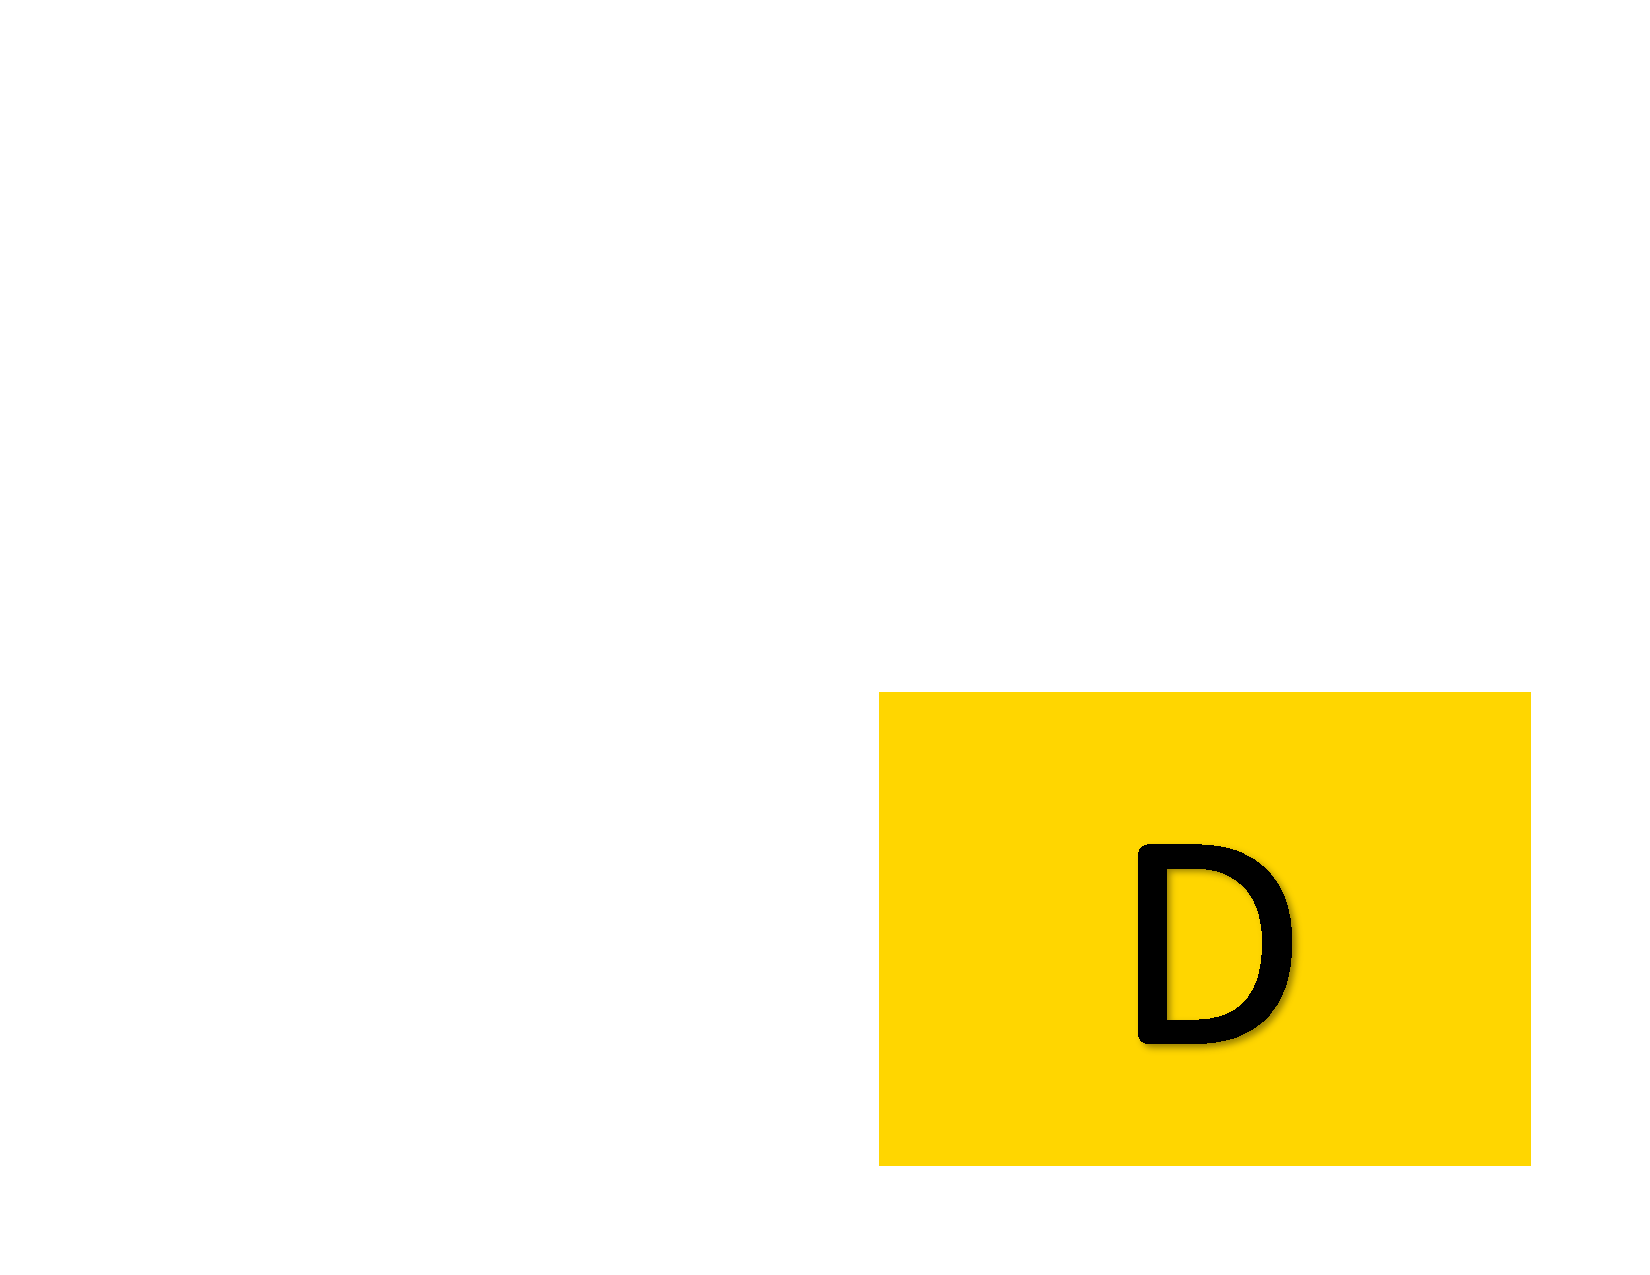
\includegraphics[width=0.8cm,height=0.5cm]{figures/D}} ]  }
\newcommand*{\eitem}{ \item[{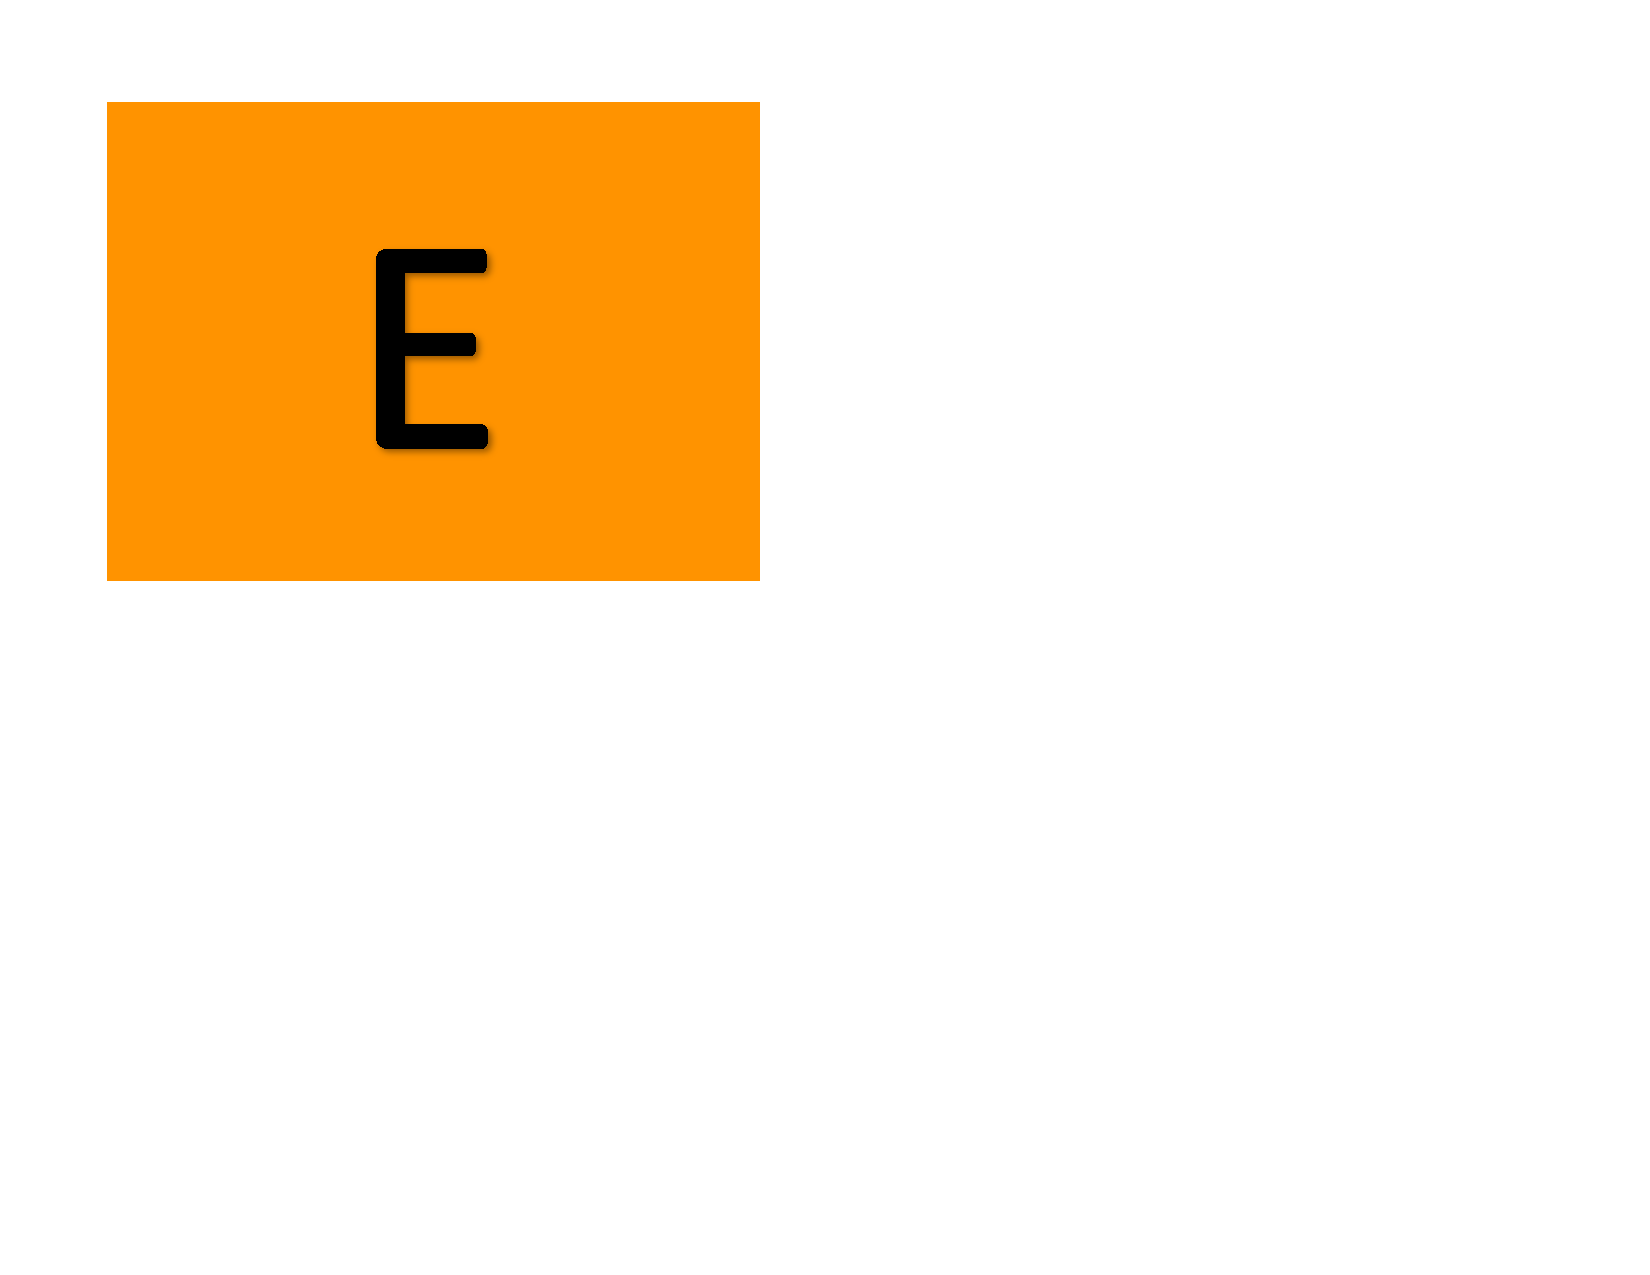
\includegraphics[width=0.8cm,height=0.5cm]{figures/E}} ]  }
\newcommand*{\fitem}{ \item[{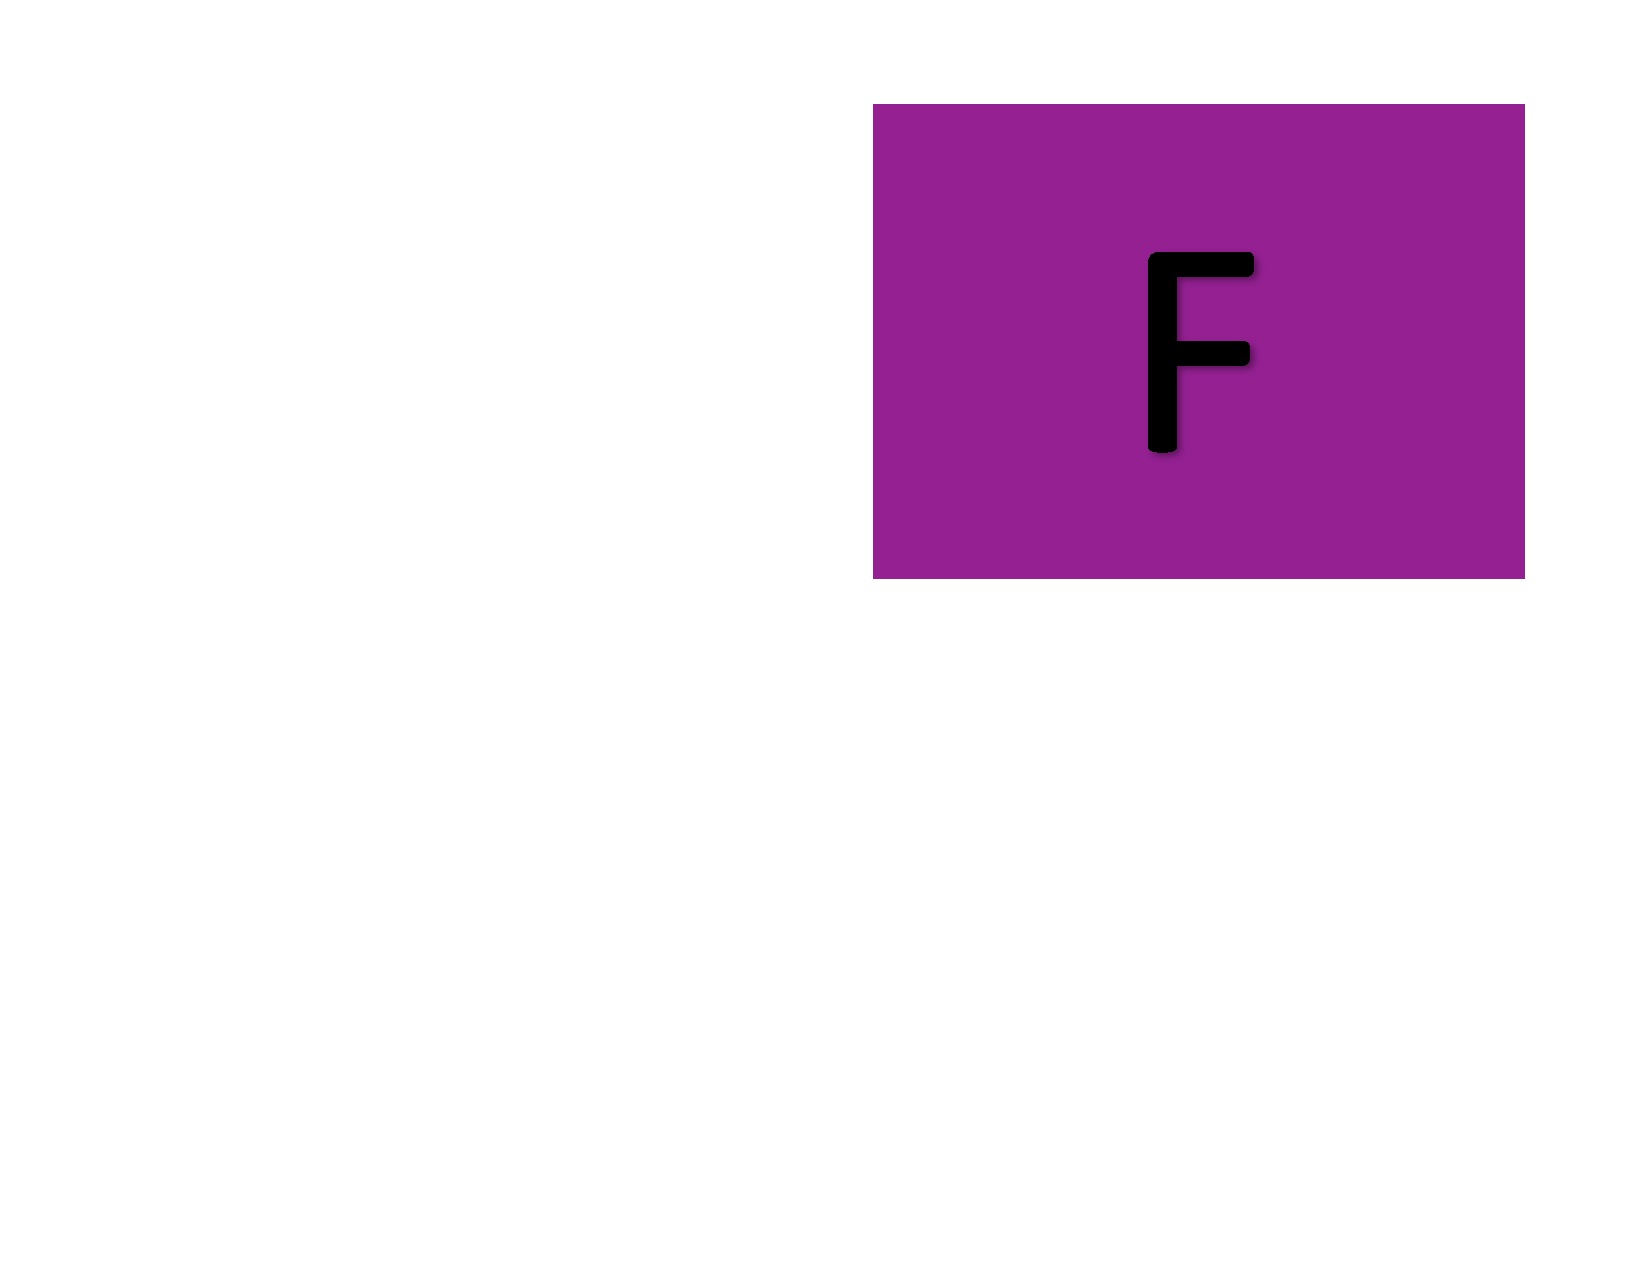
\includegraphics[width=0.8cm,height=0.5cm]{figures/F}} ]  }


\newcommand{\hide}[1]{\underline{\phantom{#1 #1}}}

\usepackage{setspace}

\onehalfspacing

\begin{document}

	\week{13, Exam 3 Review}{November 17, 2026}

	\section{Test format and instructions}

	\begin{itemize}
		\item Some multiple choice questions, some long answer questions
		\item You do not need to prove something unless you are explicitly asked to prove something
		\item You may be asked to explicitly prove something, including the correctness of a reduction or an algorithm
		\item Scratch paper will be provided
		\item No calculators or electronic devices. You will not need them. If you have to do any computations, they will be basic enough to do by hand.
		\item You will put your name on the front page, and put your initials at the top of every other page.
	\end{itemize}

	A few other notes:
	\begin{itemize}
		\item If something was on a homework or in a lecture, it could be on the test.
		\item Some questions may involve a combination of a couple different things we've seen in different lectures.
		\item If we covered a proof of a result, you can reference it as fact without re-proving it, unless the question specifically is asking you to provide proof details.
	\end{itemize}

	\newpage

	\section{Topics Covered on the Test}

	\subsection{Summary of the summary}
	\begin{itemize}
		\item Decision problems and optimization problems; polynomial time and input length
		\item Complexity classes $\mathrm{P}$, $\mathrm{NP}$, and $\mathrm{coNP}$; certificates and verifiers
		\item Polynomial-time reductions; $\mathrm{NP}$-hardness and $\mathrm{NP}$-completeness
		\item Boolean satisfiability, $\textsc{3SAT}$, $\textsc{Clique}$, and $\textsc{2SAT}$
		\item Prime factorization, primality testing, and the difference between an integer's value and its input length
		\item Undecidability and the Halting Problem
		\item Randomized algorithms: Monte Carlo and Las Vegas algorithms, and reducing error probability
		\item Hashing: collisions, universal hashing, chaining, open addressing
		\item Randomized fingerprints and the Karp--Rabin string-matching algorithm
	\end{itemize}

	For each problem or algorithm, here's the short answer on what you should know:

	\begin{itemize}
		\item How is the problem defined? Is it a decision problem, and what is its input?
		\item What does a proposed algorithm or reduction do, and why does it work?
		\item What is the running time, measured in terms of the \emph{length of the input}?
		\item What guarantees are deterministic, and what guarantees are probabilistic?
		\item Don't just know the definitions. You should know the mechanics well enough to apply them to a small example and explain the reasoning.
	\end{itemize}

	\subsection{Decision Problems and Complexity Classes}

	\begin{itemize}
		\item What is the difference between a decision problem and an optimization problem? How can an optimization problem give rise to a decision problem?
		\item What do $\mathrm{P}$, $\mathrm{NP}$, and $\mathrm{coNP}$ mean?
		\item What are a certificate and a verifier? In particular, understand the difference between a YES-certificate and a NO-certificate.
		\item Know how to show that a problem is in $\mathrm{NP}$ by describing a certificate and a polynomial-time verifier.
		\item A verifier returning NO on a bad YES-certificate does not automatically make it a NO-verifier.
		\item Know which relationships among $\mathrm{P}$, $\mathrm{NP}$, and $\mathrm{coNP}$ we can prove, and which questions are still open.
	\end{itemize}

	\subsection{Reductions and NP-Completeness}

	\begin{itemize}
		\item What does $A\leq_p B$ mean? Which problem is at least as hard as the other?
		\item If $A\leq_p B$ and $B\in\mathrm{P}$, what can you conclude? What if $A$ is $\mathrm{NP}$-complete?
		\item What is the difference between $\mathrm{NP}$-hard and $\mathrm{NP}$-complete?
		\item What are the two things you must show to prove that a problem is $\mathrm{NP}$-complete? Be sure to reduce a known $\mathrm{NP}$-complete problem \emph{to} the problem you are studying, not the other way around.
		\item Know the definitions of $\textsc{SAT}$, $\textsc{3SAT}$, $\textsc{2SAT}$, and $\textsc{Clique}$.
		\item Understand the polynomial-time reduction from $\textsc{3SAT}$ to $\textsc{Clique}$. How are vertices and edges constructed? Why does a satisfying assignment correspond to a clique?
		\item Know how the implication graph is constructed for $\textsc{2SAT}$, and how strongly connected components can be used to decide satisfiability.
		\item Remember that showing $A\leq_p B$ does \emph{not} show that $A$ is $\mathrm{NP}$-hard.
	\end{itemize}

	\subsection{Input Representation and Primality Testing}

	\begin{itemize}
		\item What is the difference between prime factorization and primality testing? Which one is a decision problem as stated?
		\item If an integer $N$ is written in binary using $n$ bits, how large can $N$ be in terms of $n$?
		\item Why is trial division up to $\sqrt{N}$ not a polynomial-time algorithm in the length of a binary input?
		\item How would this running-time analysis change if $N$ were represented in unary?
		\item Know that primality testing is in $\mathrm{P}$. Does a slow algorithm prove that a problem is not in $\mathrm{P}$?
	\end{itemize}

	\subsection{Undecidability and the Halting Problem}

	\begin{itemize}
		\item What does it mean for a decision problem to be undecidable? How is this different from being $\mathrm{NP}$-hard or $\mathrm{NP}$-complete?
		\item What is the input to the Halting Problem, and what YES or NO question are we trying to answer?
		\item Understand the contradiction proof that the Halting Problem is undecidable. In particular, why do we construct a program that does the opposite of what a hypothetical halting algorithm predicts?
		\item Why can a program's description be used as an input to another program (or to itself)?
		\item What changes if we ask whether a program halts within a specified number of steps $T$?
	\end{itemize}

	\subsection{Randomized Algorithms}

	\begin{itemize}
		\item What is the difference between a Monte Carlo algorithm and a Las Vegas algorithm?
		\item What does it mean to say that an algorithm has error probability at most $\delta$? What is random, and what is fixed?
		\item How can independent repetitions reduce the error probability of a randomized algorithm?
		\item Know the difference between expected running time, worst-case running time, and amortized running time.
	\end{itemize}

	\subsection{Hashing and Collision Resolution}

	\begin{itemize}
		\item What is a hash function? What is a collision, and why are collisions unavoidable when the universe is larger than the number of buckets?
		\item Understand the basic mechanisms of separate chaining and open addressing, including linear probing.
		\item What is the load factor $\alpha=n/B$? How does it affect search time?
		\item Know why deleting a key in an open-addressed table may require a tombstone.
		\item What does it mean for a family of hash functions to be universal?
		\item Know why universal hashing with chaining gives expected $O(1+\alpha)$ time for a fixed search. In particular, the keys and queries should be fixed independently of the randomly chosen hash function.
		\item Understand the difference between having few collisions in the entire table and having a small expected number of collisions for one fixed query.
	\end{itemize}

	\subsection{Fingerprints and Randomized String Matching}

	\begin{itemize}
		\item How can two strings be compared using short fingerprints? What kind of error can occur?
		\item Understand how a polynomial fingerprint is computed and how a rolling hash can be updated when the window shifts by one character.
		\item What does the Karp--Rabin algorithm do? Why does every true match produce a matching fingerprint?
		\item Know the running time for reporting fingerprint matches and the additional cost of explicitly verifying them.
		\item Why can randomly choosing the base make collisions unlikely? 
	\end{itemize}

	\section{Practice Problems}

	\begin{questions}

		\question What is the difference between $\mathrm{NP}$ and $\mathrm{coNP}$? Give a YES-certificate and a polynomial-time verifier for $\textsc{Clique}$. What would a NO-certificate need to establish?

		\question Let $A$ and $B$ be decision problems with $A\leq_p B$. For each statement below, say whether it must be true and briefly explain why.
		\begin{itemize}
			\item If $B\in\mathrm{P}$, then $A\in\mathrm{P}$.
			\item If $A\in\mathrm{P}$, then $B\in\mathrm{P}$.
			\item If $A$ is $\mathrm{NP}$-complete and $B\in\mathrm{NP}$, then $B$ is $\mathrm{NP}$-complete.
		\end{itemize}

		\question What are the two steps needed to prove that a decision problem $Q$ is $\mathrm{NP}$-complete? Why is proving only that $Q\in\mathrm{NP}$ insufficient?

		\question Consider the $\textsc{3SAT}$ instance
		\[
			\Phi=(x_1\vee\neg x_2\vee x_3)\wedge(\neg x_1\vee x_2\vee x_3).
		\]
		Construct the graph produced by the reduction from $\textsc{3SAT}$ to $\textsc{Clique}$. What size clique are we looking for? Find one if it exists, and explain what it tells us about $\Phi$.

		\question Explain why the reduction from $\textsc{3SAT}$ to $\textsc{Clique}$ preserves YES instances in both directions. Why are there no edges between vertices from the same clause, or between contradictory literals?

		\question Consider the following $\textsc{2SAT}$ instance:
		\[
			(x_1\vee x_2)\wedge(\neg x_1\vee x_2)\wedge(\neg x_2\vee x_1).
		\]
		Draw its implication graph and use strongly connected components to decide whether it is satisfiable.

		\question Is the following argument correct? ``Since $\textsc{2SAT}$ reduces to $\textsc{Clique}$, and $\textsc{Clique}$ is $\mathrm{NP}$-complete, $\textsc{2SAT}$ must be $\mathrm{NP}$-hard.'' Explain.

		\question Suppose that $N$ is an $n$-bit positive integer. Express the number of trial-division steps $O(\sqrt{N})$ in terms of $n$. Does this show that primality testing is not in $\mathrm{P}$? Explain.

		\question State the Halting Problem precisely. Suppose an algorithm $H$ always halts and correctly decides whether a program $M$ halts on an input $I$. Construct a program that uses $H$ to obtain a contradiction when run on its own description.

		\question Is it possible to decide whether a program halts on a given input within $T$ computation steps? Why does your answer not contradict the undecidability of the Halting Problem?

		\question Give an example of the difference between a Monte Carlo algorithm and a Las Vegas algorithm. Suppose a randomized equality test never rejects equal strings, but accepts unequal strings with probability at most $1/4$. If we run it independently three times and accept only if all three runs accept, what is the new error probability?

		\question Suppose $n$ fixed keys are hashed into $B$ buckets, with each pair colliding with probability at most $1/B$. What upper bound can you give on the expected number of colliding pairs? Why might collisions be common even when the expected cost of one search is $O(1)$?

		\question Let $B=7$, $h(x)=x\bmod 7$, and insert the keys $10,17,24,8,15,9$ into a table using separate chaining. Draw the table. What happens when we search for $31$? How does the table change when we delete $17$?

		\question Let $B=11$, $h(x)=x\bmod 11$, and insert the keys $10,21,32,4,15$ using linear probing. Show the final table. How many probes are needed to search for $43$? Why might simply marking a deleted slot as empty cause a problem?

		\question State the definition of a universal hash family. Explain why, with separate chaining, the expected running time of a fixed unsuccessful search is $O(1+n/B)$.

		\question In Karp--Rabin, suppose the text has length $n$ and the pattern has length $m$. How many candidate windows are there? How do we update a fingerprint in constant time after shifting a window one position? Why does checking every reported candidate not necessarily preserve an $O(n+m)$ running time?
	\end{questions}

\end{document}
